%%%%%%%%%%%%%%%%%%%%%%%%%%%%%%%%%%%%%%%%%%%%%%%%%%%%%%%%%%%%%%%%%%%%%%
%%                     Dissociation
%%%%%%%%%%%%%%%%%%%%%%%%%%%%%%%%%%%%%%%%%%%%%%%%%%%%%%%%%%%%%%%%%%%%%%
%\color{blue}
\subsection{Glyph: \glyph{Dissociation}}\label{sec:dissociation}

The dissociation of an \glyph{EPN} into one or more \glyph{EPNs} represents the rupture of a non-covalent binding between the biological entities represented by those \glyph{EPNs}.

\begin{glyphDescription}
 \glyphSboTerm SBO:0000180 ! dissociation.
 \glyphOrigin One \glyph{consumption} arc (\sect{consumption}).
 \glyphTarget  One or more \glyph{production} arc (\sect{production}).
 \glyphNode A \glyph{dissociation} between several entities is represented by two concentric circles. A simple empty disc could be, in some cases, confused with the \glyph{catalysis} (section \sect{catalysis}). Moreover, the existence of two circles reminds the dissociation, by contrast with the filled disc of the \glyph{association} (\sect{association}).
 \end{glyphDescription}


\begin{figure}[H]
  \centering
  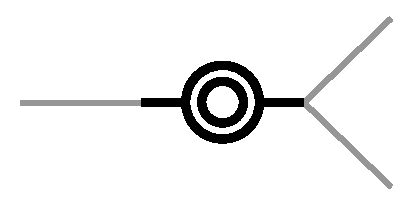
\includegraphics[scale = 0.5]{images/dissociation}
  \caption{The \PD glyph for \glyph{dissociation}.}
  \label{fig:dissociation}
\end{figure}

The example in \fig{dissoc-ribo} illustrates the dissociation of the small and large ribosomal subunits from a messenger RNA.

\begin{figure}[H]
  \centering
  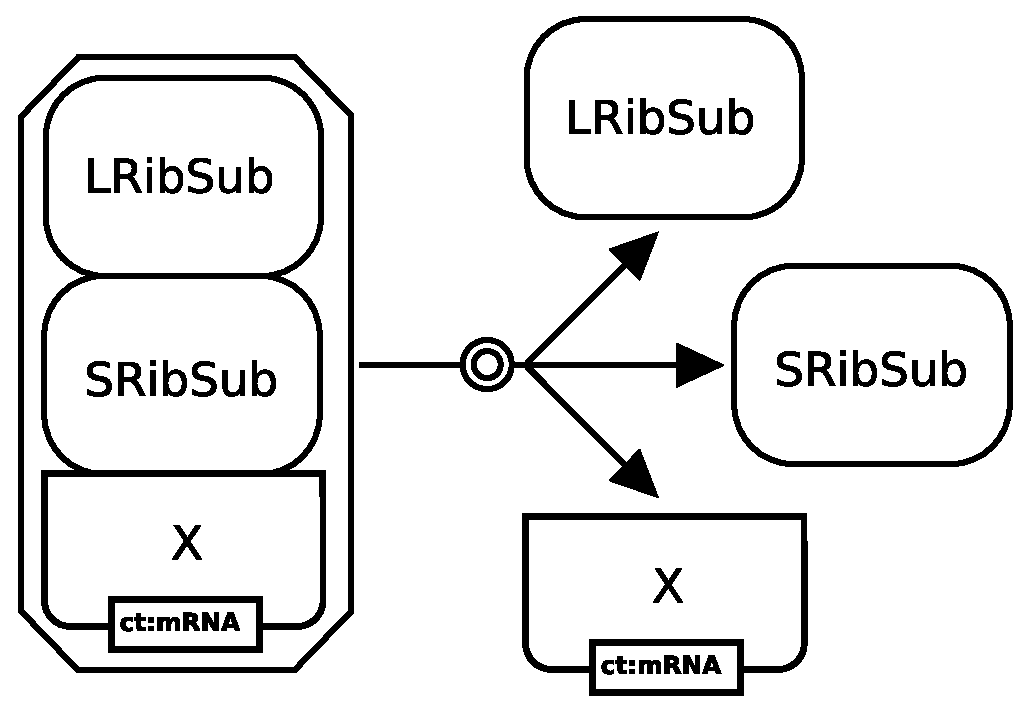
\includegraphics[scale = 0.3]{examples/dissociation-ribosome}
  \caption{Dissociation of the small and large ribosomal subunits from a messenger RNA.}
  \label{fig:dissoc-ribo}
\end{figure}
